\section{Introduction}

Some practical sections is this manual is based on the writing of
\cite{12gr730}. Going further to describe the use cases when using
AAUSHIP in a formation control setup will be described here.

The use case considered here is that of \ac{ASV} Formation Control for
Surveying Purposes. This task is about using the \ac{ASV} to scan an
area using a ``lawnmower''-pattern. This pattern is of course not a
very definite pattern, but it basically means that the mowing machine
or formation in this case will move across all the area in some way
that is structured.

\section{Description} The AAUSHIP consists of a approximately 1 metre
long vacuum formed hull made of ABS plastic, which contains twin
propellers. Additions on some AAUSHIP's include tunneltrusters for
those that want to play with those.

\begin{figure}[htbp]
	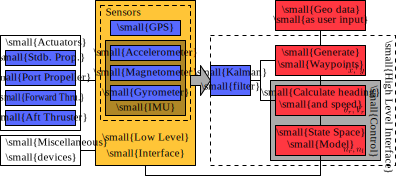
\includegraphics[width=\textwidth]{fig/vessel-block-overview}
	\caption{Overview of the control layout and its interfaces.
		Modified version of graphic from \citep{12gr730}.}
	\label{fig:vessel-block-overview}
\end{figure}
